\documentclass{article}

\usepackage{multicol}
 
\usepackage{float}

 
\usepackage[margin=0.8in]{geometry}
\usepackage{amsmath}
\usepackage{amssymb}
\usepackage{tikz}
\usepackage{natbib}
\usepackage{bbm}
\usetikzlibrary{shapes.geometric}
\usetikzlibrary{calc,positioning,shapes,arrows}
%\usepackage{natbib}
%\bibliographystyle{unsrtnat}
\newcommand{\Iota}{\mathcal{I}}

\bibliographystyle{unsrtnat}
\setlength{\columnsep}{0.8cm}

\title{Social Feedback For Robotic Collaboration}
\author{Emily Wu}

\begin{document}
\pagenumbering{gobble} 

\vspace*{8cm}

\begin{raggedleft}
	\scshape
	\huge \textbf{Social Feedback For Robotic Collaboration} \\
	\vspace{0.3cm}
	\Large 
	Emily Wu  \\
	Professor Stefanie Tellex \\
	Professor Jeff Huang \\
	Brown University \\
	May 2016 \\
\end{raggedleft}

\newpage



\vspace*{\fill}
\section*{Abstract}
Robotic collaboration requires not just communication from the human to the robot, but also from the robot to the human. We call this robot-to-human communication \emph{social feedback}. In order to flexibly and intelligently generate social feedback, we describe a Partially Observable Markov Decision Process that incorporates the human's belief about the robot's intent. We then engineer a system that can respond in near-real time that is supplemented with a multithreaded interaction model that allows for more responsive human-robot interactions. Initial evaluation in simulation shows improvement in interaction length in a toy domain and improvement in accuracy in the full domain.
\vspace*{\fill}
\newpage
\tableofcontents
\newpage
\pagenumbering{arabic} 

\maketitle
\begin{multicols}{2}
	
\section{Introduction}

Collaboration is a process that relies heavily on communication for its success. When humans collaborate, this communication is both obvious and implicit---we not only instruct and request aid from each other, but we also tacitly monitor our partners for signs of approval and understanding while producing these signals ourselves. However, in robotics, many of these vital components of successful communication are missing or lost. The absence of these signals likely account for numerous failures in human-robot collaborative tasks. In order to give robots these missing communicative skills, we employ \emph{social feedback} signals to provide human-like communication to both inform the human participant of the robot's state and request information from the participant. 

Feedback refers to the responses that are received by an agent when it takes some action. These feedback responses inform the agent about the success or failure of its actions. \emph{Social feedback} therefore refers to social signals that convey this information. These can be explicit signals, such as ``I want this object'', or implicit signals, like a perplexed expression. When humans interact with another human, they use this feedback to improve the flow and clarity of the collaboration, which in turn improves its success. For my thesis work, I have developed a framework that describes how robotic agent should likewise generate social feedback for its human partner in human-collaborative tasks, and show that it improves the speed and accuracy of human-robot interaction. 

Many existing works focus on the task of interpreting human communications\citep{tellex11,matuszek12,tellex12,misra14}, but provide no response if the interpretation fails. As a consequence, it becomes difficult to tell whether the robot is still making progress in interpreting the request, or has failed. Some works do allow for robotic responses to ambiguous situations, but the manner of their responses are hard coded, often limited to generic requests, such as ``please repeat the question''. In this work, we provide a means to generate these requests in the form of language and gesture that can flexibly represent the robot's state as well as inform the human in such a way so that allows the human to help the robot as much as possible. 

Specifically, we address the object delivery task. In this task, a set of objects are laid out on a table within a Baxter robot's reach. A human participant requests an object from the robot using speech and gesture (pointing). The robot must interpret the human's speech and gesture and deliver the requested object to the human. The task then repeats with the remaining objects on the table. This task is achievable without social feedback; the robot need only wait until enough information is given and then deliver the correct object. However, we will show that by adding social feedback actions, such as asking questions, looking at objects, and pointing at objects, we will achieve better accuracy and speed as well as improved user experience. 

\begin{figure}[H]
	\begin{center}
		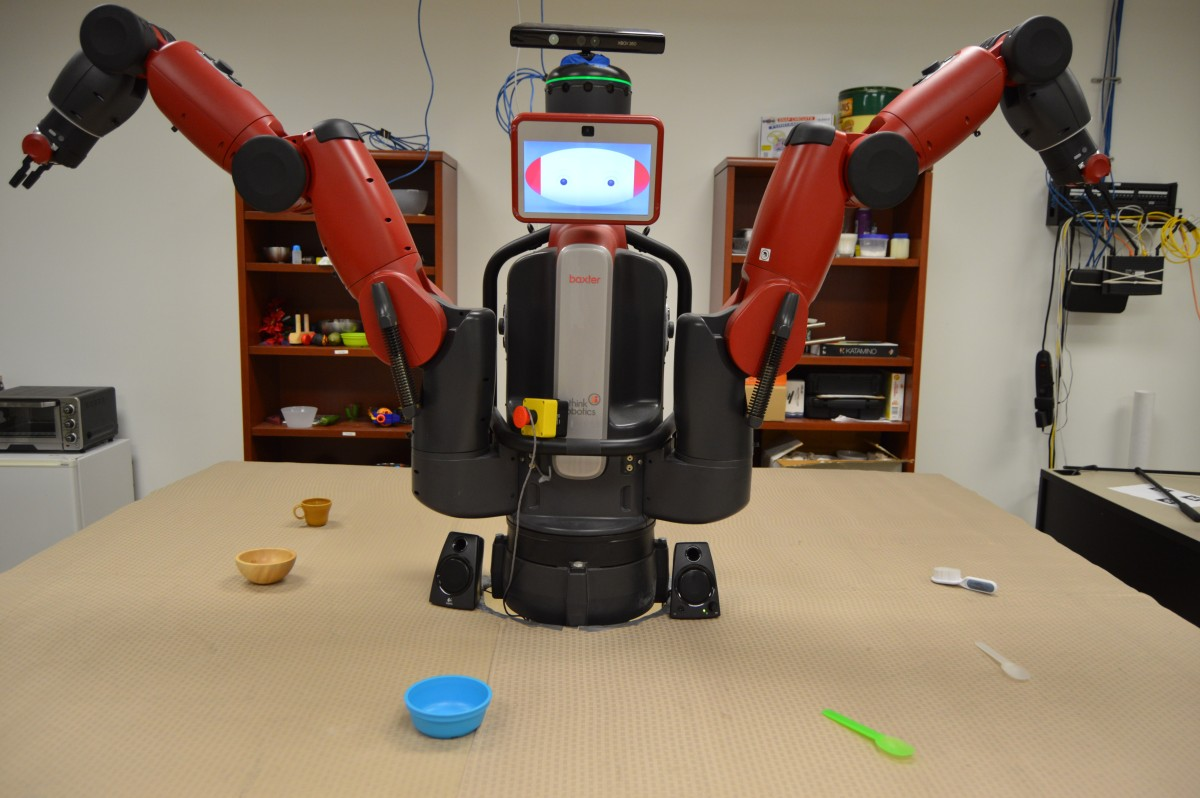
\includegraphics[scale=0.17]{firstPerson}
		\caption{The experimental setup from the participant's perspective: a Baxter robot has six objects within reach. The participant stands in front of the table to provide speech and gesture requests}
	\end{center}
\end{figure}

We will solve this problem by formulating it as a Partially Observable Markov Decision Process (POMDP)\citep{kaelbling99}, which will allow us to dynamically and flexibly determine how to choose social feedback actions. First, we will describe a two agent model and use this to motivate the construction of a POMDP. The crucial improvement we make over existing robot interaction models is that we maintain a state variable that tracks the human's interpretations of the actions the robot takes. We will next discuss how we solved this POMDP and other measures we took to allow our system to respond dynamically and fluidly. 

As an initial evaluation, we run our model in simulation to showcase improved speed and accuracy in the object delivery task. 


\section{Related Work}

This work is primarily built off of \cite{eldon15thesis}, which describes a system for incremental speech and gesture recognition in an object-delivery domain. In previous work \citep{socialfeedback}, the model from \cite{eldon15thesis} is expanded from a bayesian inference model into a POMDP model that can ask yes-no questions. In this work, we generalize the idea of the affect of robot's actions on humans state within a POMDP framework. 

Work demonstrating the importance of social feedback in human-human
communication has been done in the field of psycholinguistics. In  \cite{clark04}, one human (labeled the builder)
builds a Lego model according to instructions given by another human
(labeled the director). In the feedback-free trials, the director's
instructions were prerecorded, and the resulting models were very
inaccurate (in fact no model was completely correct). In the feedback
trials, errors were reduced by a factor of eight. Our goal is to
enable a robot to collaborate with a human in this way.


Other work with collaborative robots exists, for example, \cite{foster12} have done research with a bar-tending robot. This robot follows a rule-based state estimator, and delivers drinks from fixed positions behind the bar to multiple users based on their speech and torso position. 
We expand the scope of the problem: we do not use a rule-based state planner, our items are not in fixed positions, and our gesture model uses pointing instead of torso position. 

In \cite{bohus14},  a robotic building guide directs guests to find specific rooms. Our project addresses a similar domain, requiring the interpretation of users' requests, but differs in the task and the type of communication necessary to accomplish that task. 

Other work involving robotic object delivery also exists. Some approaches have no social feedback and will either deliver the wrong item or do nothing if given a
request it does not understand~\citep{tellex11,matuszek12,tellex12,misra14}. Language only feedback models also 
exist~\citep{chai14,macmahon06,tellex11,matuszek12,guadarrama14,hewlett11,misra14}, and several gesture only models~\citep{waldherr00,marge11}.


\cite{matuszek14} shows promising work in fusing language and complex gesture to understand references to multiple objects at once. We build off this work by including social feedback. 

In the field of computational linguistics, previous work exists in resolving referring expressions incrementally, such as~\cite{schlangen09,Zender2008Conceptual,Gieselmann}. Other work in that community also incorporates gesture, and/or eye gaze~\citep{kennington13,kennington15a}, but the given work does not incrementally update gesture along with speech. ~\cite{chairmi} provides work towards resolving referring expressions in a different domain, but does not address the task of acting on the results of these referring expressions. In~\cite{kruijffclarification}, they propose a system for planning to ask for clarifications, which covers a wide scope of knowledge failures. In this work, we are interested only in a small subset of these clarifications, and address the problem of how and when these clarifications should be used in a concrete human-robot collaboration task. 

POMDP approaches to dialog~\citep{young13} are quite common, but treat dialog
as a discrete, turn-taking interaction. The Dialog State Tracking
Challenge~\citep{williams2013dialog} a notable driving force for computer
dialog understanding, treats dialog in this turn-based way. Our model is also based off a turn-based interaction, but we provide a systems solution to allow our model to behave more incrementally.  

Interactive POMDPs (I-POMDPs)~\citep{gmytrasiewicz2005framework} describe a multi-agent POMDP that allows agents to anticipate each other's actions by forming beliefs over action and observation histories. This work attempts to accomplish the same, but makes more specialized assumptions that allow for a more tractable state space. 

Alternative approaches to
POMDPs include cognitive architecutres such as SOAR~\citep{soar} or
DIARC~\citep{diarc}.  By taking a probabilistic approach, we can seemlessly
fuse information from multiple sources and explicitly reason about the
robot's uncertainty when choosing actions.
\section{Technical Approach}

\subsection{POMDP Overview}

Partially Observable Markov Decision Processes (POMDPs) are used to model Markov Decision Processes where the true state is not known. Instead, the agent receives observations that are generated by the true state, and must infer what the true state is from the observations. Thus, the agent maintains a belief over true states which is updated as it receives new observations. The agent must then use this belief state to determine which action to take to maximize its expected value of the reward over time. This splits the POMDP into two main components, a state estimator and a policy generator. 

\paragraph{State Estimator}

The state estimator is given an initial belief and uses Bayesian mathematics to update its belief over time. In order to perform this update, the state estimator has a model of how the hidden states emit observations, called the observation function, as well as how the state evolves in response to actions performed by the robot, called the transition function. 

\paragraph{Policy Generator}

The policy generator is the means by which actions are chosen by the agent. Specifically, the policy generator should choose actions that maximize the agent's expected reward over time. The reward for taking a particular action in a state is given by a reward function. These state-action pairs are called policies, and are generated by a POMDP Solver. Generally, POMDPs are solved by converting to their equivalent belief-MDP, which is an MDP where the state is distribution over the POMDP's hidden states, a belief. In subsequent sections we will refer to this belief over states as $b$. 


Formally, a POMDP is defined as a tuple $\{S, A, T, R, \Omega, O\}$, where : 
\begin{itemize}
	\item $s \in S$ is a hidden state. 
	\item $a \in A$ is an action that an agent takes. 
	\item $T: S \times A \times S \to [0, 1]$ is a transition function that returns the value $p(s^\prime | s, a)$, the probability of transitioning to state $s^\prime \in  S$ from state $s \in S$ when taking action $a \in A$. 
	\item $R: S \times A \to \mathbb{R}$ is a reward function that returns the reward for taking action $a \in A$ in state $s \in S$. 
	\item $o \in \Omega$ is an observation. 
	\item $O: S \times A \times O \to [0, 1]$ is an observation function that returns the value of $p(o | s, a)$, the probability of observing observation $o \in O$ when action $a \in A$ transitions into $s \in S$. 
\end{itemize}

A typical bayesian network for a POMDP is provided in figure~\ref{fig:pomdp}.\footnote{In this model, we have omitted the dependency between an action and the observation from the next timestep. In the POMDP discussed in this paper, we will not use this dependency for any action. Rather, the affect of the actions on the observation is encapsulated in the state.}

\tikzstyle{h} = [circle, draw, fill=gray!40, minimum size=3em]
\tikzstyle{a} = [diamond, draw, fill=gray!40, minimum size=3em]
\tikzstyle{v} = [circle, draw, fill=white, minimum size=3em]
\tikzstyle{line} = [draw, > = stealth, -latex]


\begin{figure}[H]
\begin{center}
	\begin{tikzpicture}[node distance = 1.7cm, auto]
		%actions
		\node [v] (ort) {$o_{t}$};
		\node [a, right of=ort] (oht) {$a_{t}$};
		\node [v, right of=oht] (ortp1) {$o_{t+1}$}; 
		\node [a, left of=ort] (ohtm1) {$a_{t-1}$};
		\node [v, left of=ohtm1] (ortm1) {$o_{t-1}$};
		% states
		\node [h, above of=ort] (st) {$s_t$}; 
		\node [h, above of=ortm1] (stm1) {$s_{t-1}$}; 
		\node [h, above of=ortp1] (stp1) {$s_{t+1}$}; 
		% edges; state -> obs
		\path [line] (st) edge (ort); 
		\path [line] (stm1) edge (ortm1); 
		\path [line] (stp1) edge (ortp1); 
		% state -> state
		\path [line] (stm1) edge (st); 
		\path [line] (st) edge (stp1); 
		% a -> state
		\path [line] (ohtm1) edge (st); 
		\path [line] (oht) edge (stp1); 
	\end{tikzpicture}
\caption{A Bayesian network representation of a POMDP}
\label{fig:pomdp}
\end{center}
\end{figure}



\subsection{Model Description}

To model this human-robot interactive task, we will use a POMDP. To motivate the construction of our model, consider two-agent model constructed depicted in figure~\ref{fig:twoagent}. 

\tikzstyle{h} = [circle, draw, fill=gray!40, minimum size=3em]
\tikzstyle{v} = [circle, draw, fill=white, minimum size=3em]
\tikzstyle{line} = [draw, > = stealth, -latex]
\begin{figure}[H]
\begin{center}
	\begin{tikzpicture}[node distance = 1.5cm, auto]
		%actions
		\node [v] (ort) {$o_{t}$};
		\node [v, right of=ort] (oht) {$\omega_{\tau}$};
		\node [v, right of=oht] (ortp1) {$o_{t+1}$}; 
		\node [v, right of=ortp1] (ohtp1) {$\omega_{\tau+1}$}; 
		\node [v, left of=ort] (ohtm1) {$\omega_{\tau-1}$};
		\node [v, left of=ohtm1] (ortm1) {$o_{t-1}$};
		% states
		\node [h, above of=ort] (st) {$s_t$}; 
		\node [h, below of=oht] (sigmat) {$\sigma_\tau$};
		\node [h, above of=ortm1] (stm1) {$s_{t-1}$}; 
		\node [h, below of=ohtm1] (sigmatm1) {$\sigma_{\tau-1}$};
		\node [h, above of=ortp1] (stp1) {$s_{t+1}$}; 
		\node [h, below of=ohtp1] (sigmatp1) {$\sigma_{\tau+1}$};
		% edges; state -> obs
		\path [line] (st) edge (ort); 
		\path [line] (sigmat) edge (oht); 
		\path [line] (stm1) edge (ortm1); 
		\path [line] (sigmatm1) edge (ohtm1); 
		\path [line] (stp1) edge (ortp1); 
		\path [line] (sigmatp1) edge (ohtp1); 
		% state -> state
		\path [line] (stm1) edge (st); 
		\path [line] (st) edge (stp1); 
		\path [line] (sigmatm1) edge (sigmat); 
		\path [line] (sigmat) edge (sigmatp1); 
		% a -> state
		\path [line] (ortm1) edge (sigmatm1); 
		\path [line] (ort) edge (sigmat); 
		\path [line] (ortp1) edge (sigmatp1); 
		\path [line] (ohtm1) edge (st); 
		\path [line] (oht) edge (stp1); 
	\end{tikzpicture}
	\caption{A two-agent model based off two POMDPs}
	\label{fig:twoagent}
\end{center}
\end{figure}

We represent human states $s_t$, robot states $\sigma_\tau$, and observations generated by the robot $\omega_\tau$ and by the human $o_{t}$. Observe that the structure of this model resembles two POMDPs combined together at their actions and observations. The lower POMDP is the POMDP from the human's perspective: the robot has some hidden states $\sigma_\tau$, which the human observes by means of $\omega_{t}$. The human takes actions $o_{\tau - 1}$ to influence the robot's state $\sigma_t$. The upper POMDP models the interaction from the robot's perspective: the human's state $s_t$ is hidden from the robot, and the robot must infer it from observations $o_{t}$. When the robot takes action $\omega_{t}$, it affects the human's state $s_t$. Crucially, each agent treats the other agent's action as an observation that influences their belief about the other agent's hidden state. Thus, the human's actions affect the robot's belief about the human's state, which is what we call $b$ above. Importantly, the reverse is also true: the robot's actions affect the human's belief about what the robot's hidden state is. We will call the human's belief over the robot's hidden state $\beta$. 


In the following section we will use this dual structure to inform the construction of our POMDP as applied to our object delivery domain. 


\subsection{POMDP Definition}

We define our object-delivery POMDP as a tuple $\{S, A, T, R, \Omega, O\}$: 

\begin{itemize}
	\item Each $s \in S$ is a tuple of $\langle \iota, \beta, \Iota \rangle$		\begin{itemize}
			\item $\Iota$ is the set of all objects that the robot can deliver. Each object is parameterized by a name, a unigram vocabulary, and a position; for example: a red bowl would be represented $\langle$redBowl, [red, red, bowl, bowl, plastic], (1.0, 2.0, 0.0)$\rangle$. We assume the set of all objects is known. 
			\item $\iota \in \Iota$ is the object the human desires. This is a hidden variable. 
			\item $\beta$ is a distribution over the robot's hidden states, as defined above. In this domain, the robot state $\sigma$ represents which object the robot will hand the human, or which object the robot believes the human wants. Specifically, $\beta_t(\iota_t) = p(\iota_t | a_{1:t-1})$. While this variable is technically unknown, we make some assumptions about the transition functions and initialization so $\beta_t$'s value is known at every time step. 
		\end{itemize}
		Since our state is composed of both hidden and known states, it resembles a Mixed Observability MDP~\citep{momdp}, and we leverage the computational benefits of having both hidden and known states. 
	\item The set of actions A consists of both social and non-social actions. Non-social actions are \texttt{pick(i)} (picking up  and delivering an object $i$) and \texttt{wait}. Social actions are \texttt{point(x)}, pointing at a location $x$; \texttt{look(x)}, looking at a location $x$\footnote{$x$ is chosen from the set of points that describe the surface of the table. For computational reasons, in this work, we restrict it to the set of object locations}, and \texttt{say(p)}, informing the human that the robot believes the desired object has property $p$, where $p$ is an element of some object's vocabulary. 
	\item $T(s, a, s^\prime) = p(s^\prime | s, a)$. We make the assumption that the human's desired object $\iota$ does not change unless the robot picks up object $\iota$. The set of all objects $\Iota$ transistions to $\Iota \setminus \{i\}$ when the robot chooses action \texttt{pick(i)}. For each action in $A$, we define a ``reverse observation function'' that describes our assumptions about how the human imagines the robot generates actions (which the human sees as observations) given a hidden robot state $\sigma$. This is gone into further detail in section  \ref{sssec:tf}. 
	\item $R(s, a, s^\prime)$ returns a numeric reward from transitioning from $s$ to $s^\prime$ by taking action $a$. In this domain, we incentivize our robot to pick the correct object by giving it a +10 reward if it delivers the correct object and a -50 reward for picking the incorrect object. We also give negative rewards for taking various actions: \texttt{wait} receives a -1 reward (to incentivize the robot to finish the task quickly); \texttt{look(x)} receives a reward of -2; \texttt{say(p)} receives a reward of -3; \texttt{point(x)}  receives a reward of -4. These additional penalties for social actions reflect the penalty for ``bothering the user'', as well as the time it takes to execute these actions. These reward values were chosen experimentally to result in a high rate of pick accuracy. 
	\item Observation $o \in \Omega$ represents an observation generated by the human. These are tuples of language and gesture: $\langle l, g \rangle$. Language utterance $l$ is represented by a string of any number of words, obtained by transcribing microphone input using webkit's speech recognition API through google chrome.  A gesture $g$ is represented by a vector from the participant's shoulder to their wrist, and all gestures are interpreted as a straight-armed point. This vector is obtained using the Kinect's tracking software. 
	\item $O(o, s, a) = p(o |s, a)$ describes the probability of of seeing an observation $o$ from the human given their state $s$ and the robot's last action $a$ (though assume all observations are independent of $a$). We choose an observation function that reflects that the human is an agent attempting to communicate which object they desire to the robot, and thus chooses to generate observations that are more likely to result in the robot delivering the correct object. This is gone into more detail in the next section, section \ref{sssec:of}. 
\end{itemize}


\subsubsection{Observation Function} \label{sssec:of}

According to our double-agent model, the human emits observations as though it were an agent interacting with our robotic agent. Thus, we choose an observation model that depends on the human's belief about the robot's state, $\beta$. Specifically, the human will choose an action according to its estimate that the robot will hand them that object. In order to define this function, we will first have to define a base-level observation function. 

\paragraph{Base-Level Observation Function} \label{baseobs}

The base level observation function describes the probability of an observation conditioned only on the object: $p(o|\iota)$. For our object delivery domain, we will define two base-level observations, one for language and one for gesture. 

\vspace{0.5em}

\noindent\textit{Speech Model:} Language is interpreted according to a smoothed unigram speech model. An utterance $l$ is broken down into individual words, $w \in l$: 

\begin{equation*}
	p(l|\iota) = \prod_{w \in l} p(w|\iota) = \prod_{w\in l} \frac{\texttt{count}(w, \iota.\texttt{vocab}) + \alpha}{|\iota.\texttt{vocab}| + \alpha |\texttt{words}|}
\end{equation*}

where $\texttt{count}(w, \iota.\texttt{vocab})$ is the number of times word $w$ appears in $\iota$'s vocabulary. This allows for repeated words to have greater probability of being spoken.\footnote{In the future, object vocabularies will be collected from data; repeated words are therefore meaningful as ways that are commonly used to describe objects.}  $\alpha$ is a smoothing value chosen to be 0.05.  $|\texttt{words}|$ is the total number of words in all object vocabularies. 
\vspace{0.5em}

\noindent\textit{Gesture Model:} All gestures are interpreted as a straight armed point. These pointing gestures are selected from a normal distribution centered at the object's location. 

Define the angle between the vector defined by the pointing gesture and the vector from the human's arm to the object $\iota$ to be $\theta_\iota$. The probability of a particular gesture is then

\begin{equation*}
p(g|\iota) = \mathcal{N}(\theta_\iota | 0, v)
\end{equation*}

where $v$ is a hand-tuned variance. We choose $v = 0.4$. 

\paragraph{Posterior Observation Function}

We will use the base-level observation function defined above to define a posterior observation function that considers how the base-level observation function will affect the robot's belief. Specifically, the human chooses an action proportional to the probability that the robot will hand them the desired object $\iota$ if the human had chosen that action. The robot receives this action as an observation. 

\begin{align*}
p(o|s) = p(o|\iota, \beta) &\triangleq \eta p(\iota|o) \\
&= \eta \frac{p(o|\iota) p(\iota)}{\sum_{\iota^\prime} p(o|\iota^\prime)p(\iota^\prime)} 
\end{align*}

where $\eta$ is a normalization factor. 

Next, we will set $p(\iota) = \beta(\iota)$. $p(\iota)$ describes the robot's belief in $\iota$. This value is represented in the robot's belief-state vector, $b$. But since the human does not know $b$, it uses its estimate of $b$, $\beta$. Our new expression is 


$$p(o|s) = \eta \frac{p(o|\iota) \beta(\iota)}{\sum_{\iota^\prime} p(o|\iota^\prime)\beta(\iota^\prime)} $$

Using $\beta$ as a prior for our observation function incentivizes the robot to take actions that modify $\beta$ in such a way that increase the probability of useful observations, while in turn decreasing the probability of getting observations that tell the robot things it already knows. This result falls out of our assumption that the human is more likely to provide observations that communicate its intentions to the robot well.\footnote{It is perhaps more accurate to say that the human does not pick proportional to the probability, but picks the action with the greatest value  of $p(\iota|o)$. However, this deterministic observation function would lead to irregularities when faced with real human users who do not pick perfectly. Using a softmax function with a tuned temperature parameter would allow us to balance the strong guarantees of of a deterministic max with the flexibility of ``proportional to probability''.}  For a worked example in a toy domain, see the appendix. 



\paragraph{Modification for Object Delivery Domain}


In the object delivery domain, we have both speech and gesture, which we assume are conditionally independent given the state. 

$$p(o|s) = p(l, g | s) =  p(l|s)p(g|s)$$

In addition, it is possible to observe no speech or no gesture input. Let $L$ be a random variable that is 1 if the agent receives a language observation and 0 otherwise. Similarly, let $G$ be a random variable that is 1 if the agent receives a gesture observation and 1 otherwise. For all states $s$: 

\begin{align*}
	p(L = 1 | s) &= c_L \\
	p(L = 0 | s) &= 1 - c_L 
\end{align*}

\begin{align*}
	p(G = 1 | s) &= c_G \\
	p(G = 0 | s) &= 1 - c_G 
\end{align*}

where $c_L$ and $c_G$ are constant values less than 1. 

We will use a separate posterior observation function for language and gesture. Combined with the probability to receive a null speech or null gesture observation, the full expression is as follows: 



\begin{align*}
	p&(o|s) = \eta p(l|s) p(g|s)  \\
	&= \eta p(L|s) \left[ \frac{p(l|\iota) \beta(\iota)}{\sum_{\iota^\prime} p(l|\iota^\prime)\beta(\iota^\prime)} \right] ^ L \cdot p(G|s) \left[ \frac{p(g|\iota) \beta(\iota)}{\sum_{\iota^\prime} p(g|\iota^\prime)\beta(\iota^\prime)} \right]^G
\end{align*}




\subsubsection{Transition Function} \label{sssec:tf}

We make the assumption that every component of our state transitions conditionally independent of the other components given the previous state. In addition, each state variable depends only on its previous value and the action taken. 

\begin{align*}
	p(\iota_{t+1}&, \beta_{t+1}, \Iota_{t+1} | \iota_t, \beta_t, \Iota_t, a_t) \\
	&=  p(\iota_{t+1} | \iota_t, a_t) p(\beta_{t+1} | \beta_t, a) p(\Iota_{t+1} | \Iota_t, a_t)
\end{align*}

\paragraph{Object Transition Function}
As previously stated, we assume the object the human desires does not change unless its desired object is picked up. If the desired object is picked, it transitions uniformly at random between the remaining objects. 

If $a_t$ is \texttt{pick($\iota_t$)}, 

\begin{equation*}
	p(\iota_{t+1} | \iota_t, a_t) = \begin{cases}
		1/(|\Iota|-1) & \text{if } \iota_{t+1} \in \Iota \text{ and } \iota_{t+1} \ne \iota \\
		0 & \text{otherwise} 
	\end{cases}
\end{equation*}


If $a_t$ is any other action: 

\begin{equation*}
	p(\iota_{t+1} | \iota_t, a_t) = \begin{cases} 
		1 & \text{if $\iota_{t+1} = \iota_t$} \\
		0 & \text{otherwise}
	\end{cases}
\end{equation*}

\paragraph{Object Set Transition Function}

The set of objects $\Iota$ changes only when an object is picked up. The picked object is removed from the set. 

If $a_t$ is a \texttt{pick(i)} action: 
\begin{equation*}
	p(\Iota_{t+1} | \Iota_t, a_t) = \begin{cases}
		1 & \text{if $\Iota_{t+1} = \Iota_t \setminus \{i\}$} \\ 
		0 & \text{otherwise}
	\end{cases}
\end{equation*}


If $a_t$ is any other action: 
\begin{equation*}
	p(\Iota_{t+1} | \Iota_t, a_t) = \begin{cases}
		1 & \text{if $\Iota_{t} = \Iota_{t+1}$} \\ 
		0 & \text{otherwise}
	\end{cases}
\end{equation*}

\paragraph{Belief Transition Function}

The human's belief about which object the robot will hand over, $\beta_t$, is informed by the actions the robot takes. In the same way that the robot's belief state $b$ is a summary of all the observations the robot has made~\citep{kaelbling99}, $\beta_t$ is a summary of all observations the human has made of the robot's actions, and reflects the human's estimate about the robot's true state. We therefore update $\beta_t$ according to Bayesian probabilities in the same way that $b$ is updated. The following is a standard Markovian update: 

For a particular state $\iota_t$, its probability after $t$ observations is given as follows: 

\begin{equation*}
	p(\iota_{t+1} | o_{1:t+1}) = p(o_{t+1} | \iota_{t+1}) \sum_{\iota_{t}} p(\iota_{t+1} | \iota_{t}) p (\iota_{t} | o_{1:t})
\end{equation*}

Recall that $\beta$ is a distribution over states (objects) $\iota_t$, so we can use this rule to write an update for each entry of $\beta$. 

\begin{align*}
	\beta_{t+1}(\iota_{t+1})&= p(\iota_{t+1} | a_{1:t})  \\
	&= p(a_{t} | \iota_{t+1}) \sum_{\iota_{t}} p(\iota_{t+1} | \iota_{t}) p (\iota_{t} | a_{1:t-1}) \\ 
	&= p(a_{t} | \iota_{t+1}) \sum_{\iota_{t}} p(\iota_{t+1} | \iota_{t}) \beta_{t}(\iota_{t}) 
\end{align*}

This requires us to specify $p(a_{t} | \iota_{t+1})$. Recall that actions are operating as observations from the perspective of the human, making this expression a \emph{reverse observation function}. We must provide a reverse observation function for each action. These will often be very similar to the base-level observations described in Section \ref{sssec:of}, though adapted slightly to suit being performed by a Baxter robot. See the appendix for details. 

We must also specify a transition function, $p(\iota_{t+1} | \iota_t)$. We will use the object transition function described earlier. 

We can rewrite our element-wise update for the whole $\beta$ vector using a matrix multiplication: 


$$\beta_{t+1} = A_{t}T \beta_{t}$$


where $A_{t}$ is a matrix representing the reverse observation function $p(a_{t} | \iota_{t+1})$ and $T$ is a matrix representing the transition function $p(\iota_{t+1}|\iota_{t})$.  If the set of items $\mathcal{\iota} = \{ \iota_1, \iota_2, \ldots, \iota_n\}$, A is a diagonal such that

\begin{equation*}
	a_{ij} = \begin{cases}
		0 & \text{if } i \ne j \\
		p(a_t | \iota_{t+1} = \iota_i & \text{otherwise}
	\end{cases}
\end{equation*}

and T is a matrix with entries

\begin{equation*}
	t_{ij} = p(\iota_{t+1} = \iota_i | \iota_{t} = \iota_j)
\end{equation*}
		


This gives us a deterministic transition function for $\beta$: 

\begin{equation}
	p(\beta_{t+1} | \beta_t, a_t) = \begin{cases}
		1 & \text{if } \beta_{t+1} = A_t T \beta_t \\
		0 & \text{otherwise}
	\end{cases}
\end{equation}

If we assume that $\beta_0$ begins as the uniform distribution over objects, we can now calculate $\beta_t$ for any given time step deterministically. However, there are many assumptions that were made, and there is additional expressiveness that can be used by allowing for non-deterministic updates to $\beta$. However, we lead the exploration of this space for future work. 

\subsection{Policy Generation}

It is possible to calculate an optimal policy to solve our POMDP, however, due its size, doing so is intractable. Moreover, we would like to solve our POMDP at speeds suitable for interaction. Fortunately, approximate solutions exist which allow us to trade off accuracy for computational time. In this paper, we use the Partially Observable Sparse Sampling (POSS) algorithm \citep{Gopalan2016}, which uses Monte-Carlo Tree Search~\citep{coulom2006efficient} and Upper Confidence Bound exploration~\citep{kocsis2006bandit} to derive a policy for our POMDP. In order to improve the accuracy of the planner, we also provide a heuristic for the random rollouts that prevents the rollouts from selecting pick actions that are unlikely to select the correct objects. 

We implement this model within the Brown UMBC Reinforcement Learning And Planning~\citep{burlap} framework, which allows for many standard AI and Reinforcement learning algorithms to be used with our domain. 


\subsection{Incremental System Design}

\tikzstyle{block} = [rectangle, draw, fill=blue!20, text width=8em, text centered, rounded corners, minimum height=4em]
\tikzstyle{line} = [draw, > = stealth, -latex]

\begin{figure*}
\begin{center}
\begin{tikzpicture}[auto]
	\node [block] (st) {State Tracker}; 
	\node [left = 2.5cm of st] (n) {};
	\node [block, right = 2.5cm of st] (ap1) {Asynchronous Planner}; 
	\node [block, above = 0.5cm of ap1] (ap2) {Asynchronous Planner}; 
	\node [block, below = 0.5cm of ap1] (ap3) {Asynchronous Planner};
	\node [block, right = 2.5cm of ap1] (aq) {Action Queue};
	\path [line] (st) -- node[above] {belief state} (ap1); 
	\path [line] (st) |- node[above right, pos=0.72] {belief state} (ap2); 
	\path [line] (st) |- node[above right, pos=0.72] {belief state} (ap3); 
	\path [line] (ap1) -- node[above] {action} (aq); 
	\path [line] (ap2) -| node[above left, pos=0.22] {acton} (aq); 
	\path [line] (ap3) -| node[above left, pos=0.22] {acton} (aq); 
	\path [line] (n) -- node[above]{observations} (st);
\end{tikzpicture}
\caption{An overview of multithreaded robot interaction framework. Each node is run on a separate thread. Edges are labeled with the type of data transmitted}
\label{fig:system}. 
\end{center}
\end{figure*}

Interactive systems that involve speech often make an assumption that the interaction can be split neatly into turns: first one speaker provides a complete utterance, and then the other. This is often not the case, and it is a subtle matter to determine when one turn is completed and the other agent can begin to speak. As a consequence, many systems involving dialogue, including earlier iterations of this project, do not ``hear'' utterances or gestures while the agent is speaking or acting. Any speech or gestures the human made while the robot was executing its action were dropped and never incorporated into the robot's belief about the state. An additional problem was that while the robot was planning its next action, it would also not incorporate any observations made. This was a significant effect, as it could take up to 10 seconds of planning for the robot to make its next move. As a consequence, most observations would be dropped unless we incorporated a system of turn-taking where we waited a set amount of time for the human to provide any speech and gesture input. 

While turn-taking is an adequate solution for dialogue-only systems, full fledged interaction is more continuous. Even when speaking in a turn-like manner, agents give signals back and forward to signal their understanding and also provide corrections and interruptions.

In order to create more fluid interactions, we employ a multithreaded solution that separates the state estimation, planning, and executions of actions. This allows our robot to simultaneously track the human's belief, plan its next move, and interact with the human. A diagram of the system is available in figure~\ref{fig:system}





\paragraph{State Tracker} The state tracker incorporates observations from the human at a very high rate, allowing the tracker to always have access to the most up to date state estimation. However, our domain description requires the robot to choose an action between each consecutive observation. We address this by feeding the model a \texttt{wait} action unless the planning thread has provided a different action. This requires minimal dependency between actions and observations, which our model avoids. 

\paragraph{Asynchronous Planner} A separate thread runs the planning code. Planning can take several seconds, during which the robot is not only idle, but also deaf and blind. Running the planning code on a separate thread allows the robot to continue observing and interacting with the human while the robot plans its next move. In addition, we can use several planning threads at once, with separate policies to control the robot's face, arms, head angle, etc. In our work, we use one thread to plan for the POMDP domain described above, and another to animate the Baxter's face to show and facial expression of increasing confusion with the entropy of the belief state. 

\paragraph{Action Queue} The planning threads push their actions onto a queue which executes them one by one, allowing the planning threads to resume planning if the actions they produce take some time to execute. An additional advantage is that this allows the robot to be constantly acting, with minimal idle time. 

\section{Evaluation}

Due to difficulties with the POSS algorithm, we return to Belief Sparse Sampling~\citep{bss} (BSS) to evaluate the efficacy of our model. BSS, however, takes several minutes to generate an action, which is too slow for user interaction. Instead, we evaluate the performance of our model in simulation. A procedure for user studies with human participants is also described.\footnote{We do note that it would be possible to run the full domain in real time to test with users by precomputing and caching a policy for each belief state that describes the optimal action to take from that state. This is the scheme that we used in \cite{socialfeedback}}

\subsection{Results in Simulation}

To evaluate the performance of our model, we run simulated trials with two different domains: first with a toy domain, and second with the full social feedback domain. 
\subsubsection{Toy Domain Results}

The toy domain is a simplified version of the full social feedback domain. Objects are represented by binary string bits of length 3, and observations tell the robot that a particular bit has some value. There is no noise in observations. The agent can take \texttt{wait} and \texttt{pick} actions in the non-social trials, and in the social trials, can take non-social actions as well as actions of the form \texttt{inform(x, y)}, which represents informing the human that the robot believes that the $x$th digit has value $y$. 

We run 25 trials in simulation. Results are presented in figure \ref{fig:toyresults}. We see a sharp reduction in the number of actions needed until the robot can successfully pick the correct object, while accuracy remains the same. In this simple domain, it is easy to identify the correct object with enough observations, accounting for the high accuracy in both domains. However, taking social feedback actions allows the agent to request the observations that it needs from the human to complete the interaction as quickly as possible. Notice also that the variance in the number of actions the robot takes until the first correct pick is very small in the social trials, while it is very large in the non-social trials. Social feedback actions allow the agent to control the interaction so that it is as brief as possible. 

\begin{figure}[H]
\begin{center}
	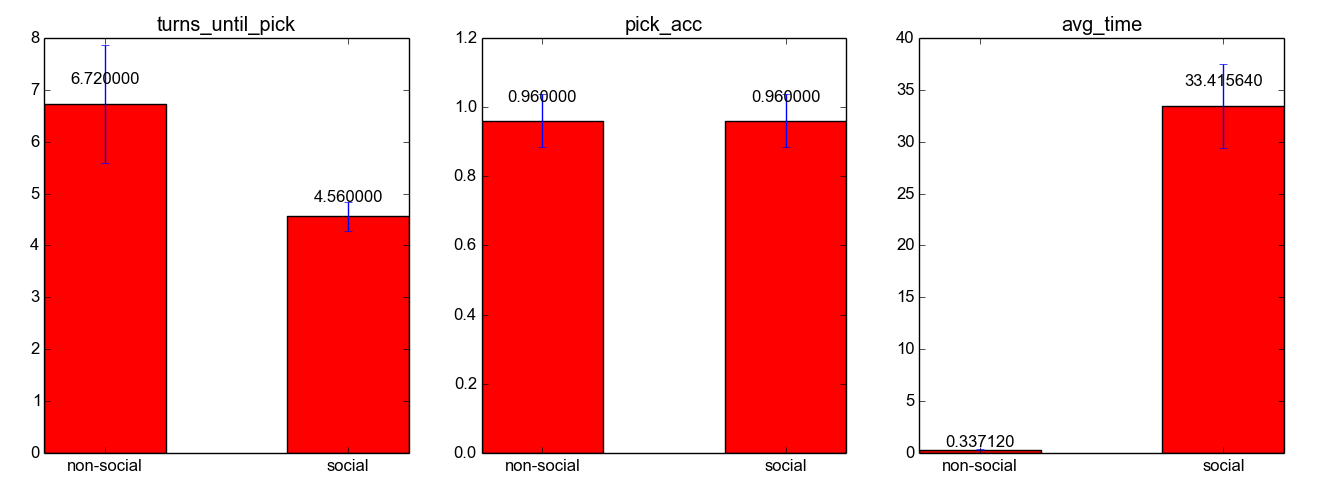
\includegraphics[width=0.45\textwidth]{toy_results}
\end{center}
\caption{Results in simulation for the toy domain. \texttt{turns\_until\_pick} is the number of timesteps until first correct pick,  \texttt{pick\_acc} is the ratio of correct picks to total picks}
	\label{fig:toyresults}
\end{figure}

\subsubsection{Full Domain Results}


We run two simulated trials: one without any social feedback actions (only \texttt{pick(i)} and \texttt{wait}), and one with non-social feedback actions and a random subset of six social feedback actions (to reduce computation time). There are four objects on the table for each trial. Each trial uses a different set of randomized actions (to reduce computation costs). Results are presented in figure \ref{fig:results}. 

We see a small, but statistically significant improvement in accuracy at the cost of slightly less than one additional action for the first correct pick. The less pronounced effects of social feedback are likely due to the greater number of observations that are possible, and the relative probability of seeing a useful observation is reduced. This more complicated domain is also hampered by our reduced horizon of 2, allowing the planner to only consider up to two actions in the future. In the full domain, the agent is much less likely to receive enough observations to correctly pick the object within two timesteps, even using social feedback actions. 

To see more improvement in speed and accuracy, we would likely need to use a larger planning horizon, which is only possible with approximate solvers such as POSS. In addition, increasing the number of objects, i.e., the complexity of the task, would likely result in a sharper difference between the number of turns required to give the human the correct object. The robot is unlikely to receive a useful observation unless it can signal to the human which observation it requires. 



\begin{figure}[H]
\begin{center}
	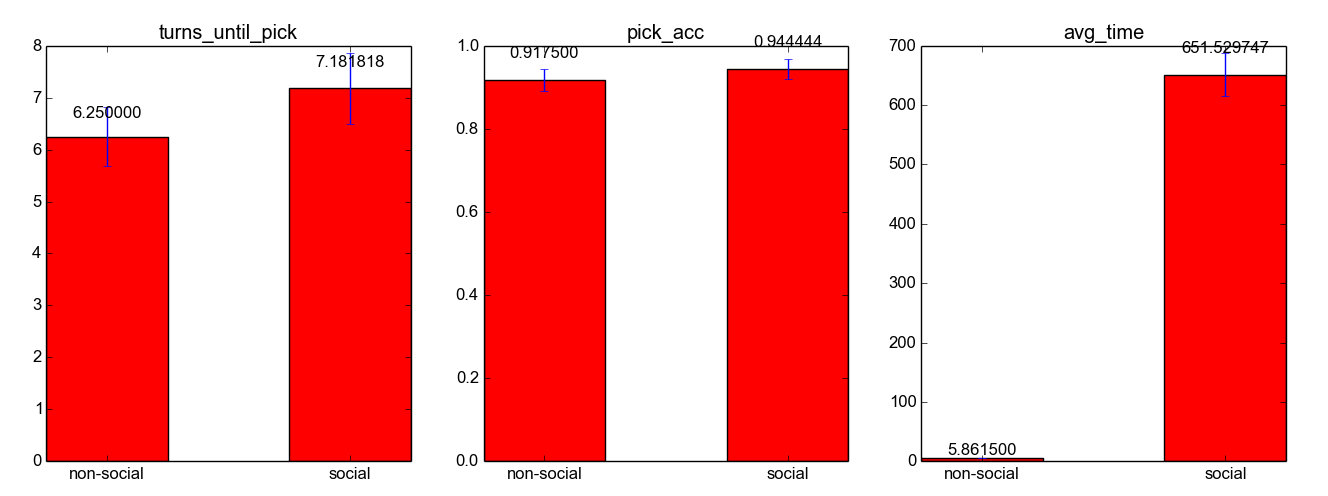
\includegraphics[width=0.45\textwidth]{full_results}
\end{center}
\caption{Results in simulation for the full domain. \texttt{turns\_until\_pick} is the number of timesteps until first correct pick,  \texttt{pick\_acc} is the ratio of correct picks to total picks}
	\label{fig:results}
\end{figure}

\subsection{User Studies Procedure}

Users are acquired from convenience sampling by inviting volunteers from the Brown University CIT building. For each user, two trials are run: a baseline trial without any social feedback actions, and a social-feedback trial with social feedback actions enabled. For each trial, the user is given a microphone and invited to use speech and gesture to ask the robot for a specific item on the table, and to not change that object until it was picked up. After their requested object is picked up, they request a new object and repeat the procedure until the robot has handed them all objects on the table. It is decided randomly whether the social or non-social trial is performed first for each user. Between the two trials, they are given a survey to assess the qualitative aspects of the interaction, including metrics such as the robot's perceived intelligence, friendliness, etc. 

This procedure is based off a previous user study run for an earlier iteration of this project. In this user study, we noticed a small effect showing the increased speed of interaction with social feedback actions enabled. However, this study was run with only six participants, so these effects were likely not statistically significant. When user studies are run in the future, we will have a larger sample size, but also increase the difficulty of the task by adding more objects, which should further highlight the necessity of social feedback. 

Interesting metrics to measure include are how the perception of the robot is correlated to the actions the robot takes, as well as the accuracy and speed of the interaction. We may also consider a longer-running user study to investigate how people learn how to interact with the robot. 



\section{Future Work}

The next task will be to run user-studies with human participants to compare the performance of the system with and without social feedback. This will require the exploration of approximate solvers to allow us to solve the POMDP in real time, or to precompute policies. 

We would also like to expand the domain by allowing for more modalities of user input, such as other types of gestures as well as more subtle cues such as expression or emotion. In the same vein, more exploration can be done in the area of robot expression, investigating more types of social feedback action and formalizing how they affect human belief. 

Other areas for further exploration can be found by removing many of the assumptions made in this thesis. For example, the set of objects on the table was assumed to be known. Attempting to learn from the human more about the set of objects, such as their vocabularies and location, would be an interesting expansion. 

Use of the $\beta$ variable can be expanded to include uncertainty over the value of $\beta_t$, allowing for ambiguity in how the human interprets the robot's action. In the same vein, additional modes of interaction from both the robot and human can be explored. 

The object delivery domain can also be abstracted to a domain where the goal is not to determine which object the human wants, but the human's intent in general. This system of tracking the human's belief about the robot's communicated intent can be widely applied to other human-robot interaction tasks. 



\section{Acknowledgements}

This thesis is the result of work that has been ongoing since December 2014. I would like to acknowledge my many collaborators, Advik Guha, Miles Eldon, David Whitney, Horatio Han, Nakul Gopalan, Lawson Wong, James MacGlashan, and John Oberlin. 

This project is part of an ongoing initiative towards social robotics by Brown University's H2R laboratory under Professor Stefanie Tellex. 

\end{multicols}

\newpage
\section{Appendix}

\subsection{Posterior Observation Function: Toy Example}
In order to demonstrate and motivate the posterior observation function, we will define a toy domain. In this toy domain, the states are the following: $\{AA, AB, BA, BB\}$ as well as $\beta$, which is a distribution over these states. The observations are $\{A\_, \_A, B\_, \_B\}$, which mean ``the first character is an A'', ``the second character is an A'', ``the first character is B'', ``and the second character is a B'' respectively. These observations are provided by the human. The agent can take actions $CX$ which is informing the human that the agent believes the Xth character is a C, as well as ``picking'' the object or waiting. For the basel level observation, the human always gives truthful observations, and has equal probability of generating an observation pertaining to a particular character. We will see how this affects the POMDP observation function, which incorporates $\beta$. 

Consider the following situation: 

Intially both $b$, the robot's belief about the human's desired object and $\beta$, the human's belief about the robot's belief, are uniform. The true state is $AA$. 

\begin{center}
\begin{tabular}{|c| c| c| c | c|}
	\hline
	$t$ & $b$ & $\beta$ & $a$ & $o$ \\
	\hline
	$0$ & [0.25, 0.25, 0.25, 0.25] & [0.25, 0.25, 0.25, 0.25] & & \\
	\hline
\end{tabular}
\end{center}


The robot then receives an observation $A\_$. The new beliefs are: 

\begin{center}
\begin{tabular}{|c| c| c| c | c|}
	\hline
	$t$ & $b$ & $\beta$ & $a$ & $o$ \\
	\hline
	$0$ & [0.25, 0.25, 0.25, 0.25] & [0.25, 0.25, 0.25, 0.25] & & \\
	\hline
	$1$ & [0.50, 0.50, 0, 0] & [0.25, 0.25, 0.25, 0.25] & & $A\_$ \\
	\hline
\end{tabular}
\end{center}

Next, the robot can choose to take an action. If it chooses to wait, this is the resulting state


\begin{center}
\begin{tabular}{|c| c| c| c | c|}
	\hline
	$t$ & $b$ & $\beta$ & $a$ & $o$ \\
	\hline
	$0$ & [0.25, 0.25, 0.25, 0.25] & [0.25, 0.25, 0.25, 0.25] & & \\
	\hline
	$1$ & [0.50, 0.50, 0, 0] & [0.25, 0.25, 0.25, 0.25] & & $A\_$ \\
	\hline
	$2$ & [0.50, 0.50, 0, 0] & [0.25, 0.25, 0.25, 0.25] & wait  &  \\
	\hline
\end{tabular}
\end{center}

Examine the probabilities of each observation.

\begin{align*}
	p(A\_ | AA, \beta) &= \frac{ p(A\_)\beta(AA) }{ p(A\_)\beta(AA) + p(A\_)\beta(AB) + p(A\_)\beta(BA) + p(A\_)\beta(BB)} \\
	&= \frac{0.5 * 0.25}{0.5 * 0.25 + 0.5 * 0.25 + 0 + 0} \\
	&= 0.5
\end{align*}

\begin{align*}
	p(\_A | AA, \beta) &= \frac{ p(\_A)\beta(AA) }{ p(\_A)\beta(AA) + p(\_A)\beta(AB) + p(\_A)\beta(BA) + p(\_A)\beta(BB)} \\
	&= \frac{0.5 * 0.25}{0.5 * 0.25 + 0 + 0.5 * 0.25 + 0} \\
	&= 0.5
\end{align*}

The probabilities of all other actions are 0, since we only give truthful observations.

Notice that this situation is not ideal. The agent has equal probabilities of receiving either observation, even though the agent already knows that the first character is an A. Now, consider what would happen if the robot chose the action $A0$. We would get the following belief states: 


\begin{center}
\begin{tabular}{|c| c| c| c | c|}
	\hline
	$t$ & $b$ & $\beta$ & $a$ & $o$ \\
	\hline
	$0$ & [0.25, 0.25, 0.25, 0.25] & [0.25, 0.25, 0.25, 0.25] & & \\
	\hline
	$1$ & [0.50, 0.50, 0, 0] & [0.25, 0.25, 0.25, 0.25] & & $A\_$ \\
	\hline
	$2$ & [0.50, 0.50, 0, 0] & [0.5, 0.5, 0, 0] & $A0$  &  \\
	\hline
\end{tabular}
\end{center}

If we examine the probabilities again: 

\begin{align*}
	p(A\_|AA, \beta) &\propto \frac{ p(A\_)\beta(AA) }{ p(A\_)\beta(AA) + p(A\_)\beta(AB) + p(A\_)\beta(BA) + p(A\_)\beta(BB)} \\
	&\propto \frac{0.5 * 0.5}{0.5 * 0.5 + 0.5 * 0.5 + 0 + 0} \\
	&\propto 0.5 \\
	&= \frac{1}{3}
\end{align*}

\begin{align*}
	p(\_A|AA, \beta) &\propto \frac{ p(\_A)\beta(AA) }{ p(\_A)\beta(AA) + p(\_A)\beta(AB) + p(\_A)\beta(BA) + p(\_A)\beta(BB)} \\
	&\propto \frac{0.5 * 0.5}{0.5 * 0.5 + 0 + 0 + 0} \\
	&\propto 1 \\
	&= \frac{2}{3}
\end{align*}
 
Now, we are more likely to get the observation $\_A$, which is more useful to us than the observation $A\_$, since it gives us the information we need to pick the correct object, $AA$. This provides an incentive for the robot to choose an action that conveys something about its current state of belief over doing nothing. 

\subsection{Reverse Observation Functions}

We define a reverse observation function for each action the robot can take. These define how $\beta$ is updated when a robot takes an action. 

For $\texttt{look(x)}$ actions, we define an angle $\phi_l$ to be the angle between a vector from the robot's face to the location $x$ and the vector from the robot's face to the location of object $\iota_{t+1}$. We assume this angle is chosen from a normal distribution centered at 0 with a hand tuned variance, $v_l$. 
$$p(a_{t} = \texttt{look(x)} | \iota_{t+1}) = \mathcal{N}(\phi_l | 0, v_{l})$$

For $\texttt{point(x)}$ actions, we define an angle $\phi_p$ to be the angle between the vector from Baxter's wrist to location $x$ and the vector from Baxter's wrist joint to the object $\iota_{t+1}$. This gesture is chosen according to a normal distribution with hand-tuned variance $v_p$. 

$$p(a_{t} = \texttt{point(x)} | \iota_{t+1}) = \mathcal{N}(\phi_p | 0, v_{p})$$

Actions $\texttt{say(p)}$ take the form of a statement ``I believe that the object you want is $p$'', where $p$ is some property from some object's vocabulary. The probability of this action given some $\iota$ is identical to the speech model for the human, given in section~\ref{baseobs}. 

\newpage

\bibliography{main}


\end{document}
